\documentclass[10pt,letterpaper]{hmcpset}
\usepackage[margin=1in]{geometry}
\usepackage{graphicx}
\usepackage{amsthm}
\usepackage{enumitem}
\usepackage{amsmath}
\usepackage{amsmath,amssymb,amsfonts}
\usepackage{algorithmic}
\usepackage{hyperref}
\usepackage{graphicx}
\usepackage{textcomp}
\usepackage{algorithm}
\usepackage{booktabs}
\usepackage{algorithmic}
\usepackage{enumitem}
\usepackage{subfig}
\usepackage{xcolor, cancel}
\usepackage{color,soul}
\setlength{\parindent}{0 pt}
\setlength{\parskip}{1 em}
\usepackage{hyperref}
\hypersetup{
colorlinks=true,
linkcolor=blue,
filecolor=magenta,      
urlcolor=cyan,
}

% Theorems
\usepackage{amsthm}
\renewcommand\qedsymbol{$\blacksquare$}
\makeatletter
\@ifclassloaded{article}{
    \newtheorem{definition}{Definition}[section]
    \newtheorem{example}{Example}[section]
    \newtheorem{theorem}{Theorem}[section]
    \newtheorem{corollary}{Corollary}[theorem]
    \newtheorem{lemma}{Lemma}[theorem]
}{
}
\makeatother

% Random Stuff
\setlength\unitlength{1mm}

\newcommand{\insertfig}[3]{
\begin{figure}[htbp]\begin{center}\begin{picture}(120,90)
\put(0,-5){\includegraphics[width=12cm,height=9cm,clip=]{#1}}\end{picture}\end{center}
\caption{#2}\label{#3}\end{figure}}

\newcommand{\insertxfig}[4]{
\begin{figure}[htbp]
\begin{center}
\leavevmode \centerline{\resizebox{#4\textwidth}{!}{\input
#1.pstex_t}}
\caption{#2} \label{#3}
\end{center}
\end{figure}}

\long\def\comment#1{}

\newcommand\abs[1]{\left\lvert#1\right\rvert}
\newcommand\norm[1]{\left\lVert#1\right\rVert}
\DeclareMathOperator*{\argmin}{arg\,min}
\DeclareMathOperator*{\argmax}{arg\,max}

% bb font symbols
\newfont{\bbb}{msbm10 scaled 700}
\newcommand{\CCC}{\mbox{\bbb C}}

\newfont{\bbf}{msbm10 scaled 1100}
\newcommand{\CC}{\mbox{\bbf C}}
\newcommand{\PP}{\mbox{\bbf P}}
\newcommand{\RR}{\mbox{\bbf R}}
\newcommand{\QQ}{\mbox{\bbf Q}}
\newcommand{\ZZ}{\mbox{\bbf Z}}
\renewcommand{\SS}{\mbox{\bbf S}}
\newcommand{\FF}{\mbox{\bbf F}}
\newcommand{\GG}{\mbox{\bbf G}}
\newcommand{\EE}{\mbox{\bbf E}}
\newcommand{\NN}{\mbox{\bbf N}}
\newcommand{\KK}{\mbox{\bbf K}}
\newcommand{\KL}{\mbox{\bbf KL}}

% Vectors
\renewcommand{\aa}{{\bf a}}
\newcommand{\bb}{{\bf b}}
\newcommand{\cc}{{\bf c}}
\newcommand{\dd}{{\bf d}}
\newcommand{\ee}{{\bf e}}
\newcommand{\ff}{{\bf f}}
\renewcommand{\gg}{{\bf g}}
\newcommand{\hh}{{\bf h}}
\newcommand{\ii}{{\bf i}}
\newcommand{\jj}{{\bf j}}
\newcommand{\kk}{{\bf k}}
\renewcommand{\ll}{{\bf l}}
\newcommand{\mm}{{\bf m}}
\newcommand{\nn}{{\bf n}}
\newcommand{\oo}{{\bf o}}
\newcommand{\pp}{{\bf p}}
\newcommand{\qq}{{\bf q}}
\newcommand{\rr}{{\bf r}}
\renewcommand{\ss}{{\bf s}}
\renewcommand{\tt}{{\bf t}}
\newcommand{\uu}{{\bf u}}
\newcommand{\ww}{{\bf w}}
\newcommand{\vv}{{\bf v}}
\newcommand{\xx}{{\bf x}}
\newcommand{\yy}{{\bf y}}
\newcommand{\zz}{{\bf z}}
\newcommand{\0}{{\bf 0}}
\newcommand{\1}{{\bf 1}}

% Matrices
\newcommand{\Ab}{{\bf A}}
\newcommand{\Bb}{{\bf B}}
\newcommand{\Cb}{{\bf C}}
\newcommand{\Db}{{\bf D}}
\newcommand{\Eb}{{\bf E}}
\newcommand{\Fb}{{\bf F}}
\newcommand{\Gb}{{\bf G}}
\newcommand{\Hb}{{\bf H}}
\newcommand{\Ib}{{\bf I}}
\newcommand{\Jb}{{\bf J}}
\newcommand{\Kb}{{\bf K}}
\newcommand{\Lb}{{\bf L}}
\newcommand{\Mb}{{\bf M}}
\newcommand{\Nb}{{\bf N}}
\newcommand{\Ob}{{\bf O}}
\newcommand{\Pb}{{\bf P}}
\newcommand{\Qb}{{\bf Q}}
\newcommand{\Rb}{{\bf R}}
\newcommand{\Sb}{{\bf S}}
\newcommand{\Tb}{{\bf T}}
\newcommand{\Ub}{{\bf U}}
\newcommand{\Wb}{{\bf W}}
\newcommand{\Vb}{{\bf V}}
\newcommand{\Xb}{{\bf X}}
\newcommand{\Yb}{{\bf Y}}
\newcommand{\Zb}{{\bf Z}}

% Calligraphic
\newcommand{\Ac}{{\cal A}}
\newcommand{\Bc}{{\cal B}}
\newcommand{\Cc}{{\cal C}}
\newcommand{\Dc}{{\cal D}}
\newcommand{\Ec}{{\cal E}}
\newcommand{\Fc}{{\cal F}}
\newcommand{\Gc}{{\cal G}}
\newcommand{\Hc}{{\cal H}}
\newcommand{\Ic}{{\cal I}}
\newcommand{\Jc}{{\cal J}}
\newcommand{\Kc}{{\cal K}}
\newcommand{\Lc}{{\cal L}}
\newcommand{\Mc}{{\cal M}}
\newcommand{\Nc}{{\cal N}}
\newcommand{\Oc}{{\cal O}}
\newcommand{\Pc}{{\cal P}}
\newcommand{\Qc}{{\cal Q}}
\newcommand{\Rc}{{\cal R}}
\newcommand{\Sc}{{\cal S}}
\newcommand{\Tc}{{\cal T}}
\newcommand{\Uc}{{\cal U}}
\newcommand{\Wc}{{\cal W}}
\newcommand{\Vc}{{\cal V}}
\newcommand{\Xc}{{\cal X}}
\newcommand{\Yc}{{\cal Y}}
\newcommand{\Zc}{{\cal Z}}

% Bold greek letters
\newcommand{\alphab}{\hbox{\boldmath$\alpha$}}
\newcommand{\betab}{\hbox{\boldmath$\beta$}}
\newcommand{\gammab}{\hbox{\boldmath$\gamma$}}
\newcommand{\deltab}{\hbox{\boldmath$\delta$}}
\newcommand{\etab}{\hbox{\boldmath$\eta$}}
\newcommand{\lambdab}{\hbox{\boldmath$\lambda$}}
\newcommand{\epsilonb}{\hbox{\boldmath$\epsilon$}}
\newcommand{\nub}{\hbox{\boldmath$\nu$}}
\newcommand{\mub}{\hbox{\boldmath$\mu$}}
\newcommand{\zetab}{\hbox{\boldmath$\zeta$}}
\newcommand{\phib}{\hbox{\boldmath$\phi$}}
\newcommand{\psib}{\hbox{\boldmath$\psi$}}
\newcommand{\thetab}{\hbox{\boldmath$\theta$}}
\newcommand{\taub}{\hbox{\boldmath$\tau$}}
\newcommand{\omegab}{\hbox{\boldmath$\omega$}}
\newcommand{\xib}{\hbox{\boldmath$\xi$}}
\newcommand{\sigmab}{\hbox{\boldmath$\sigma$}}
\newcommand{\pib}{\hbox{\boldmath$\pi$}}
\newcommand{\rhob}{\hbox{\boldmath$\rho$}}

\newcommand{\Gammab}{\hbox{\boldmath$\Gamma$}}
\newcommand{\Lambdab}{\hbox{\boldmath$\Lambda$}}
\newcommand{\Deltab}{\hbox{\boldmath$\Delta$}}
\newcommand{\Sigmab}{\hbox{\boldmath$\Sigma$}}
\newcommand{\Phib}{\hbox{\boldmath$\Phi$}}
\newcommand{\Pib}{\hbox{\boldmath$\Pi$}}
\newcommand{\Psib}{\hbox{\boldmath$\Psi$}}
\newcommand{\Thetab}{\hbox{\boldmath$\Theta$}}
\newcommand{\Omegab}{\hbox{\boldmath$\Omega$}}
\newcommand{\Xib}{\hbox{\boldmath$\Xi$}}

% mixed symbols
\newcommand{\sinc}{{\hbox{sinc}}}
\newcommand{\diag}{{\hbox{diag}}}
\renewcommand{\det}{{\hbox{det}}}
\newcommand{\trace}{{\hbox{tr}}}
\newcommand{\tr}{\trace}
\newcommand{\sign}{{\hbox{sign}}}
\renewcommand{\arg}{{\hbox{arg}}}
\newcommand{\var}{{\hbox{var}}}
\newcommand{\cov}{{\hbox{cov}}}
\renewcommand{\Re}{{\rm Re}}
\renewcommand{\Im}{{\rm Im}}
\newcommand{\eqdef}{\stackrel{\Delta}{=}}
\newcommand{\defines}{{\,\,\stackrel{\scriptscriptstyle \bigtriangleup}{=}\,\,}}
\newcommand{\<}{\left\langle}
\renewcommand{\>}{\right\rangle}
\newcommand{\Psf}{{\sf P}}
\newcommand{\T}{\top}
\newcommand{\m}[1]{\begin{bmatrix} #1 \end{bmatrix}}


% info for header block in upper right hand corner
\name{Joseph Gardi, Nathan Schroeder}
\class{Differential Geometry}
\assignment{Homework 5}

\renewcommand{\labelenumi}{{(\alph{enumi})}}

\begin{document}

\subsection*{ Read: } 

\begin{itemize}
\item{Baby Do Carmo, Differential Geometry
of Curves and Surfaces:  
Sections 2-2, 2-3, 2-4 and  Appendix (starting on page 118) on A Brief
Review of Continuity and Differentiability}
\item{Handouts 6 and 7}
\item{Lecture Notes}
\end{itemize}

\subsection*{ Do: }
Remember, the problems marked with an asterisk have hints in the back of the book. Additionally, many of these problems ask that you re-prove something that do Carmo proves in the reading.

\textbf{A: Problems on Reviewing of Continuity and Differentiability}\\
\begin{problem}
a) Prove the proposition 7 on page 127, Baby Do Carmo.

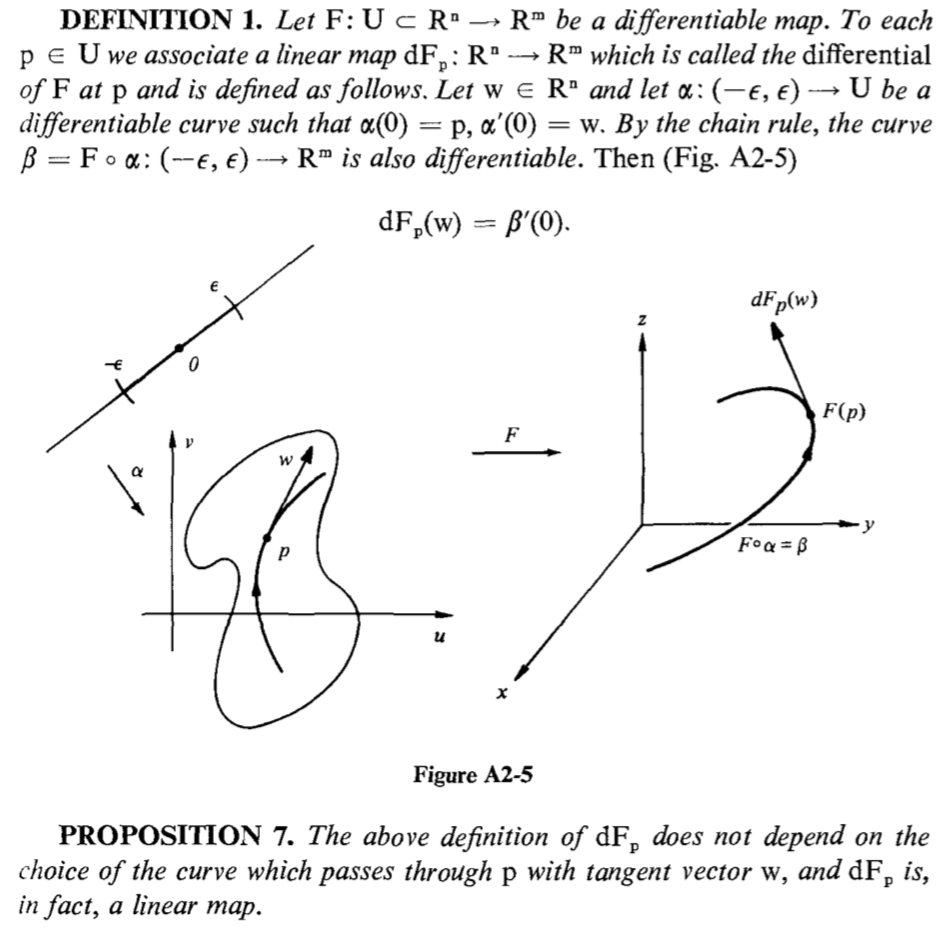
\includegraphics[scale=0.7]{Aa.png}
\end{problem}
\begin{solution}
\end{solution}

\newpage \begin{problem}
b) Prove the proposition 8 on page 129, Baby Do Carmo.

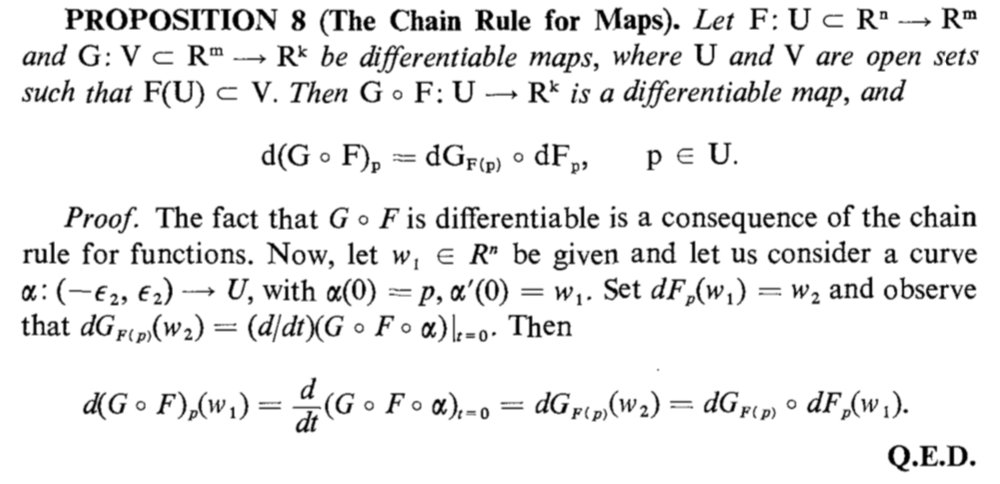
\includegraphics[scale=0.7]{Ab.png}
\end{problem}
\begin{solution}
\end{solution}

\newpage \begin{problem}
c) Rewrite Example 11 on page 132 of Baby Do Carmo and explain 
clearly why the Inverse Function Theorem (page 131) is true only in a neighborhood of a point $p$. 

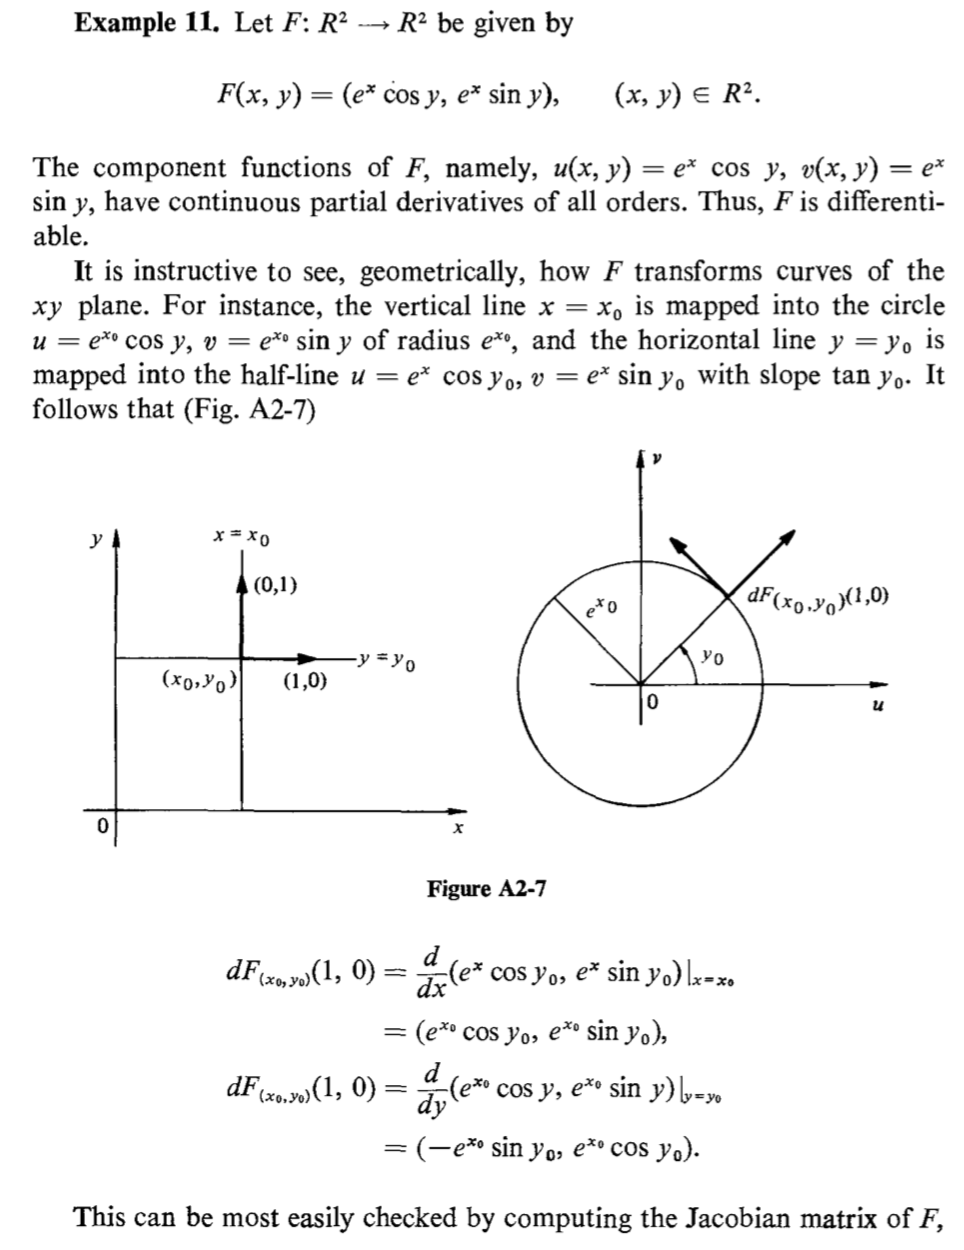
\includegraphics[scale=0.7]{Ac1.png}
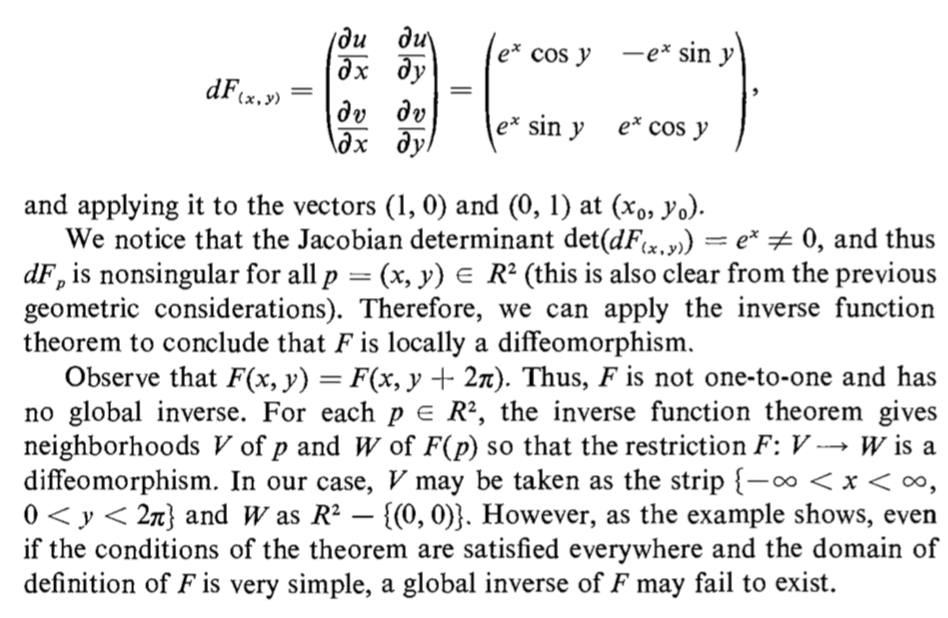
\includegraphics[scale=0.7]{Ac2.png}
\end{problem}
\begin{solution}
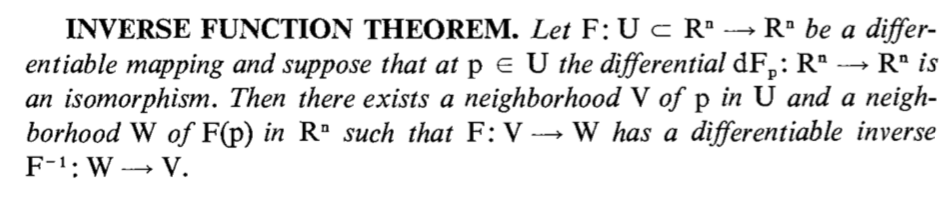
\includegraphics[scale=0.7]{Ac0.png}
\end{solution}

\newpage \begin{problem}
d) Show that an infinite cylinder after deleting a vertical line is 
diffeomorphic to a plane.
\end{problem}
\begin{solution}
%First observe that any two infinite cylinders are diffeomorphic. Indeed given two infinite cylinders a rigid motion applied to one of them will reduce the problem to that of
%showing that any two infinite cylinders with a common axis are diffeomorphic. Another
%application of a rigid motion will further reduce the problem to that of showing that any
%two cylinders centered about the z-axis are diffeomorphic. In this later case, a dilation will
%map one onto the other. Clearly rigid motions and dillations are diffeomorphisms. The
%upshot of these observations is that we may establish the result in general by establishing
%a specific case.
%The specific case we consider is the infinite cylinder with diameter 2 centered along the
%line through the point $(0, 0, 1)$ and parallel to the y-axis. We remove the line through the
%point $(0, 0, 2)$ and parallel to the y-axis. A cross section of this cylinder at some fixed y0
%is pictured in the figure. We map this punctured circle onto the line through the point
%$(0, y0, 0)$ and parallel to the x-axis via ”stereographic projection”.
%We claim that the map
%\begin{align*}
%F(x, y, z) = (\frac{2x}{2 - z}, y)
%\end{align*}
%defines a diffeomorphism between the cyllinder with the line removed and the plane.

Let r be the radius of the cylinder and put the center of the cylinder at the
origin.

Let the plane be $span([1, 0, 0], [0, 1, 0])$. \\
Let's use something like cylindrical coordinates. We are parameterizing the infinite
cylinder with $\alpha: (\theta, h) \rightarrow (r \cos \theta, r \sin \theta,h)$. Proving that this is a
parameterization is left as an excersise.  \\

Let $x: (a, b) \rightarrow (2\pi \frac{|a|}{|a| + 1}, b)$. \\
I want to show that $\alpha \circ x}$ is a difeomorphism between the plane and the
cylinder. To do this it is sufficient to show that $x$ is diffeomorphic since
 is a parameterization .
It is left as an excersise to show that $x$ is a bijection. Now to show that
it is differentiable and has differentiable inverse we show that the jacobian
is invertable at all points in the plane. Let $(a, b, c) \in \mathbb{R}^3$ be given. \\
The jacobian is,
\begin{align*}
  &\begin{bmatrix}
    \frac{\partial x_1}{\partial a} & \frac{\partial x_1}{\partial b} \\
    \frac{\partial x_2}{\partial a} & \frac{\partial x_2}{\partial b} \\
  \end{bmatrix} \\
  &= \begin{bmatrix}
    2\pi \cdot \frac{1 - |a|/(|a|+1)}{|a|+1} & 0 \\
    0 & 1 \\
  \end{bmatrix}
\end{align*}
Now we just need to show this matrix is invertable for all $a$.
The determinant is 
\begin{align*}
  2\pi \cdot \frac{1 - |a|/(|a|+1)}{|a|+1}
\end{align*}
The determinant approaches zero but never actually reaches it so $x$ is diffeomorphic.
\end{solution}


\newpage 
\textbf{B: Problems from Lectures}\\
\begin{problem}
a) Use Inverse Function Theorem to give a proof 
of proposition 2, page 59, Baby Co Carmo.

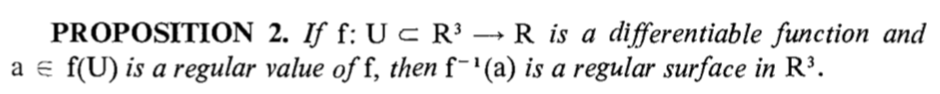
\includegraphics[scale=0.7]{Ba.png}
\end{problem}
\begin{solution}
\end{solution}

\newpage \begin{problem}
b) Use Inverse Function Theorem to give a proof 
of proposition 4, page 64, Baby Co Carmo.

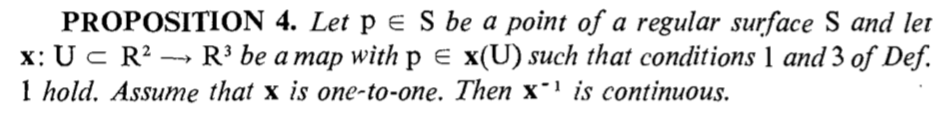
\includegraphics[scale=0.7]{Bb.png}
\end{problem}
\begin{solution}
\end{solution}


\newpage
\textbf{C: Other Problems}\\
\begin{problem}
a) Problem 7 on page 66, Section 2-2, Baby Do Carmo.

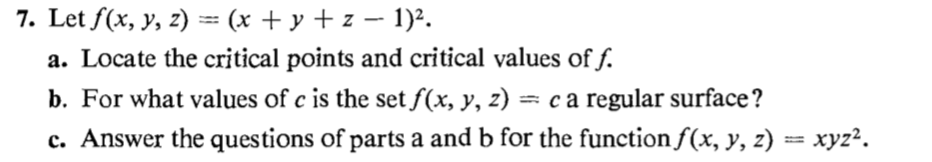
\includegraphics[scale=0.7]{Ca.png}
\end{problem}
\begin{solution}
  First we find the set of critical points $C = \{ (x, y, z) \in \mathbb{R}^3 :
  \mathbf{d}f(x, y, z) = 0\}$ 
  So for each $(x, y, z) \in C$,
  \begin{align*}
    &\mathbf{d}f(x, y, z) = 0 \\
    \iff &\begin{bmatrix}2(x + y + z - 1) & 2(x + y + z - 1) & 2(x + y + z - 1)\end{bmatrix} = 0 \\
    \iff &x + y + z - 1 = 0 
  \end{align*}
  This is the equation of a plane. So $C$ is the set of points in a plane. The
  critical values are the image $f(C) = \{ f(x, y, z): (x, y, z) \in C \} = \{ (x + y + z - 1)^2 : x + y + z - 1 = 0 \}
  = \{ 0 \}$
\end{solution}

\newpage \begin{problem}
b) Problem 11 on page 66, Section 2-2, Baby Do Carmo.

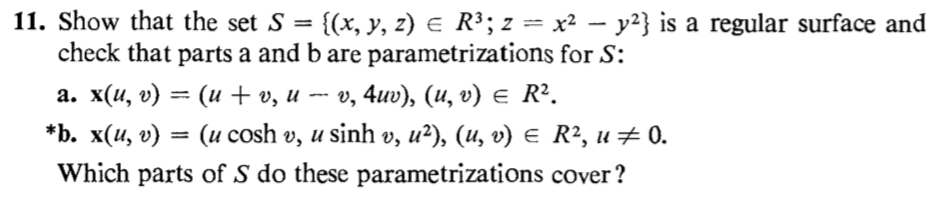
\includegraphics[scale=0.7]{Cb.png}
\end{problem}
\begin{solution}
%  This regular surface can be described with the function $f(x, y) = x^2 - y^2$
%  so that $S = \{ f(x, y) : (x, y) \in \mathbb{R}^2 \}$. $f$ is
%  differentiable and regular everywhere so $S$ is a regular surface.  \\
%  To show that $f$ is regular everywhere observe that $\mathbb{b}f(x, y)
%  = \begin{bmatrix}2x & -2y\end{bmatrix}$.
%  We can prove that if a set can be described as a differntiable
%  function it is a regular surface because the parameterization would just be
%  $(x, y) \rightarrow (x, y, f(x, y))$. This parameterization is differentiable everywhere 

I'll do both part $a$ and part $b$ at once.
To show that $a, b$ are reegular you can show that the differential for both
functions is invertable. So for $a$  the differential is,
\begin{align*}
  \mathbf{d}a(u, v) = \begin{bmatrix}
    1 & 1 \\
    1 & -1 \\
    4v & 4u
  \end{bmatrix}
\end{align*}
This matrix is an invertable map everywhere because it has the minor 
$\begin{bmatrix}1&1\\1&-1\end{bmatrix}$ which is  not invertable. \\
Similarly, for $b$,
\begin{align*}
  \mathbf{d}b(u, v) = \begin{bmatrix}
    \cosh v & u \sinh v \\
    \sinh v & u \cosh v \\
    2u & 0 
  \end{bmatrix}
\end{align*}
It was given that $u \neq 0$ for inputs to $b$ so $2u$ is not a multiple of $0$.
Therefore, the columns of $\mathbf{d}b$ are always linearly independent. So
the map is always invertable. \\

Now let's show that the images
of both functions are contained in $S$. let's call the functions $a, b$ rather
than calling both of them $x$. For all $p =(u + v, u - v, 4uv) \in
x(\mathbb{R}^2)$, $(u + v)^2 - (u - v)^2 = u^2 + 2uv + v^2 - (u^2 - 2uv + v^2)
= 4uv$. So $z = x^2 - y^2$ is satisified for at $p$. Therefore $p \in S$.
Similarly for $b$:
\begin{align*}
  \forall p = (u \cosh v, u \sinh v, u^2) \in image(b), \\
  (u \cosh v)^2 - (u \sinh v)^2 = u^2(\cosh^2 v - \sinh^2 v) = u^2
\end{align*}
To show that $a, b$ are homeomorphic we have to show they are bijective. First I
do it for $a$. Suppose that $a(u_1, v_1) = a(u_2, v_2)$. Then I will show that
$u_1, = u_2, v_1, = v_2$. This gives us the matrix equation,
\begin{align*}
  A\begin{bmatrix}u_1\\v_1\end{bmatrix} = A \begin{bmatrix}u_2\\v_2\end{bmatrix} \\
  \implies \begin{bmatrix}u_1\\v_1\end{bmatrix} =  \begin{bmatrix}u_2\\v_2\end{bmatrix} &\text{(because $A$ is invertible)}\\
  \text{where } A = \begin{bmatrix}1&1\\1&-1\end{bmatrix}
  \end{align*}
  Showing $b$ is bijective is left as an excersise.
  Then to show that $a, b$ are homeomorphic we observe that they are continuous
  and have continuous inverses. 
 To Show that the $x$ covers $V \bigcap S$ for some neighborhood $V \subset S$ just . 
\end{solution}

\newpage \begin{problem}
c) Problem 1 on page 80, Section 2-3, Baby Do Carmo.

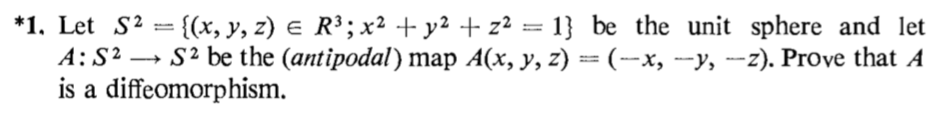
\includegraphics[scale=0.7]{Cc.png}
\end{problem}
\begin{solution}
 First observe it is a bijection. Then observe that the jacobian is inverable everywhere.
\end{solution}

\newpage \begin{problem}
  d) Problem 8 on page 80, Section 2-3, Baby Do Carmo. \\

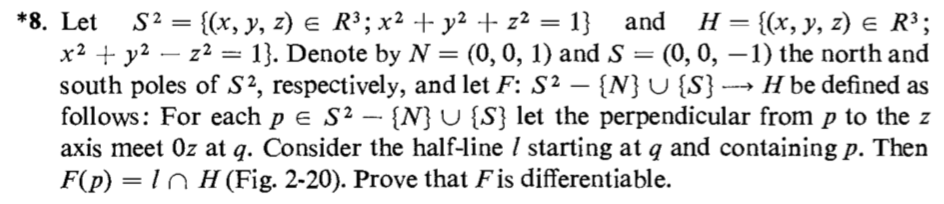
\includegraphics[scale=0.7]{Cd.png}
\end{problem}
\begin{solution}
  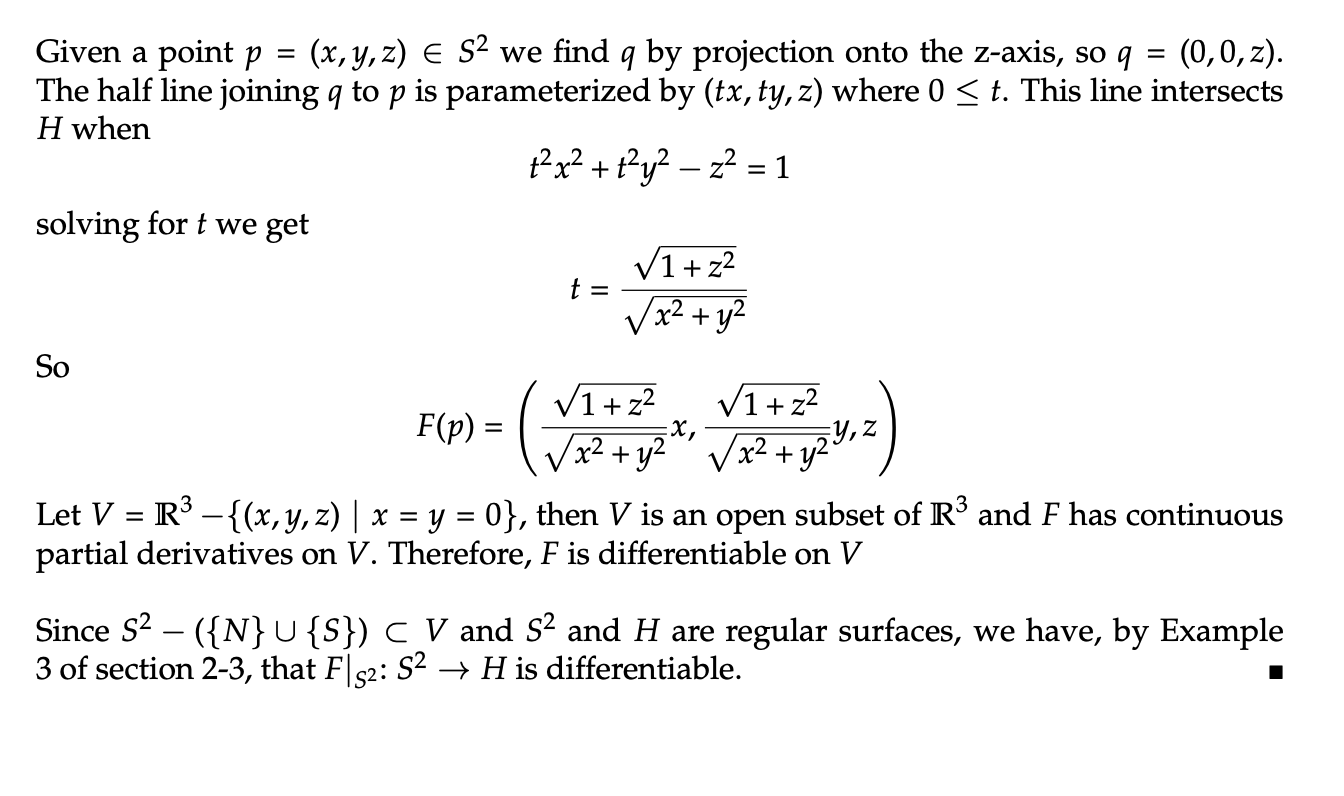
\includegraphics[scale=.8]{d_solution.png}
\end{solution}

\newpage \begin{problem}
e) Problem 10 on page 81, Section 2-3, Baby Do Carmo.

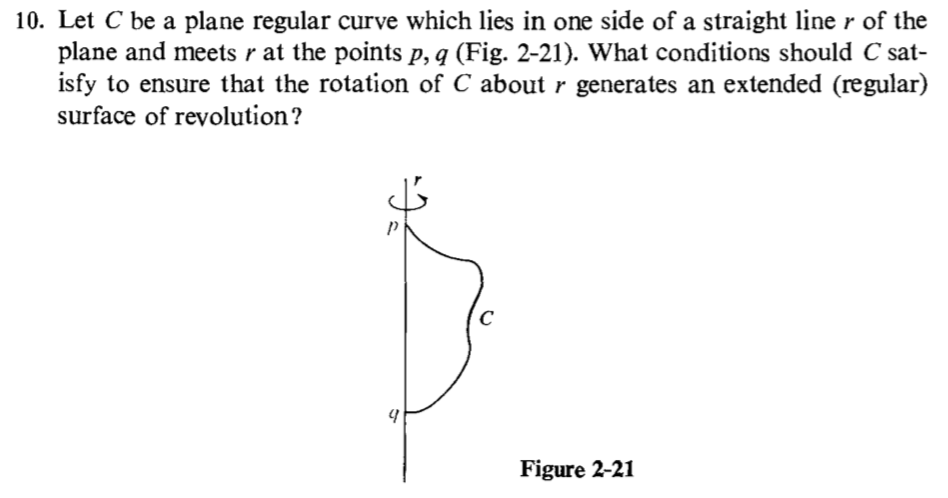
\includegraphics[scale=0.7]{Ce.png}
\end{problem}
\begin{solution}
  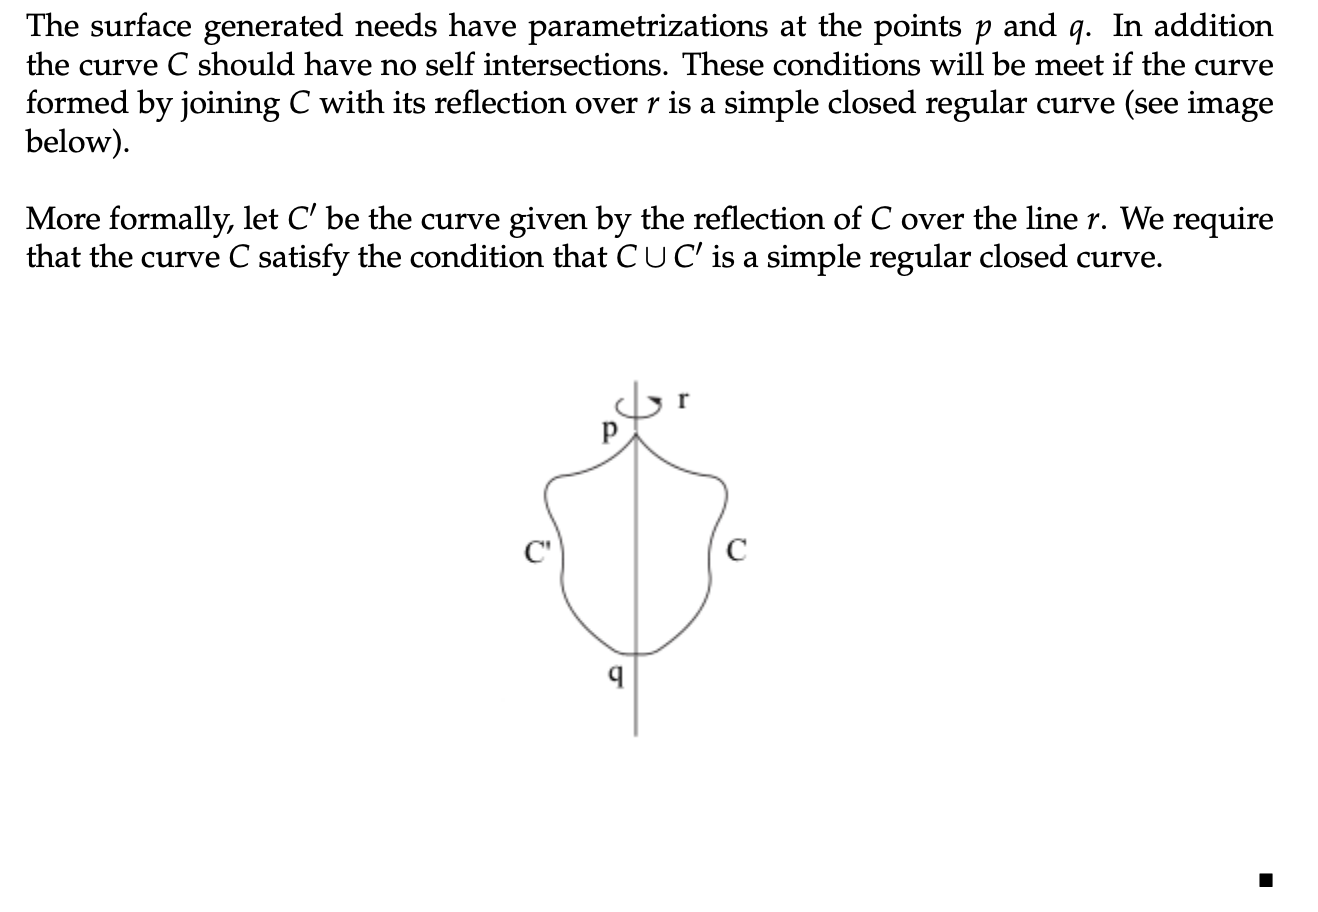
\includegraphics[scale=.8]{e_solution.png}
\end{solution}

\newpage \begin{problem}
f) Problem 12 on page 81, Section 2-3, Baby Do Carmo.

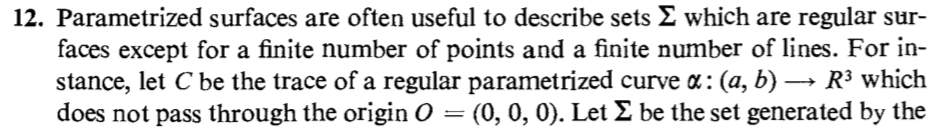
\includegraphics[scale=0.7]{Cf1.png}
\end{problem}
\begin{solution}
\end{solution}

\newpage \begin{problem}
f continued) 

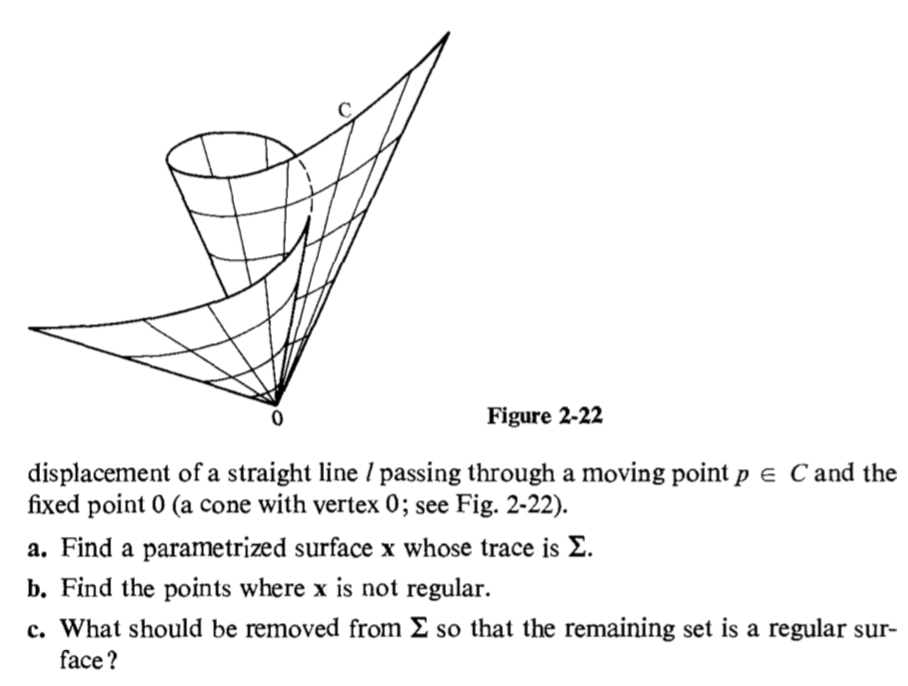
\includegraphics[scale=0.7]{Cf2.png}
\end{problem}
\begin{solution}
  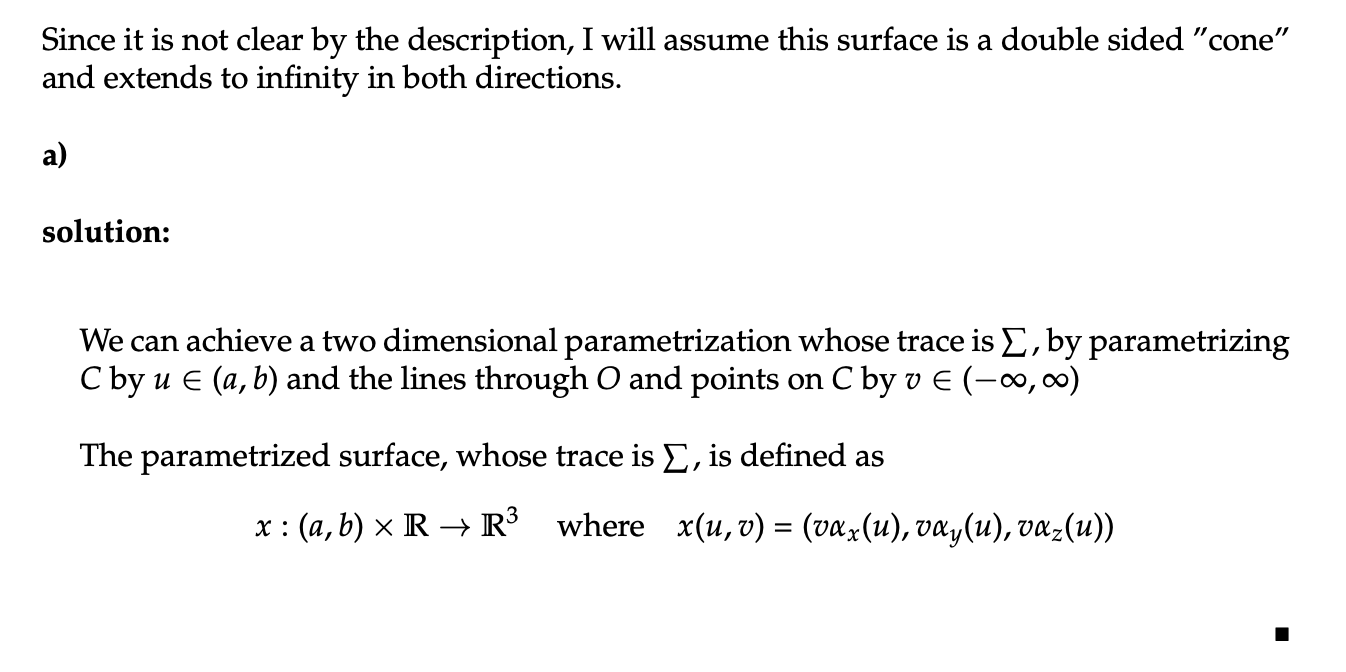
\includegraphics[scale=.8]{C_f1_solution.png}
  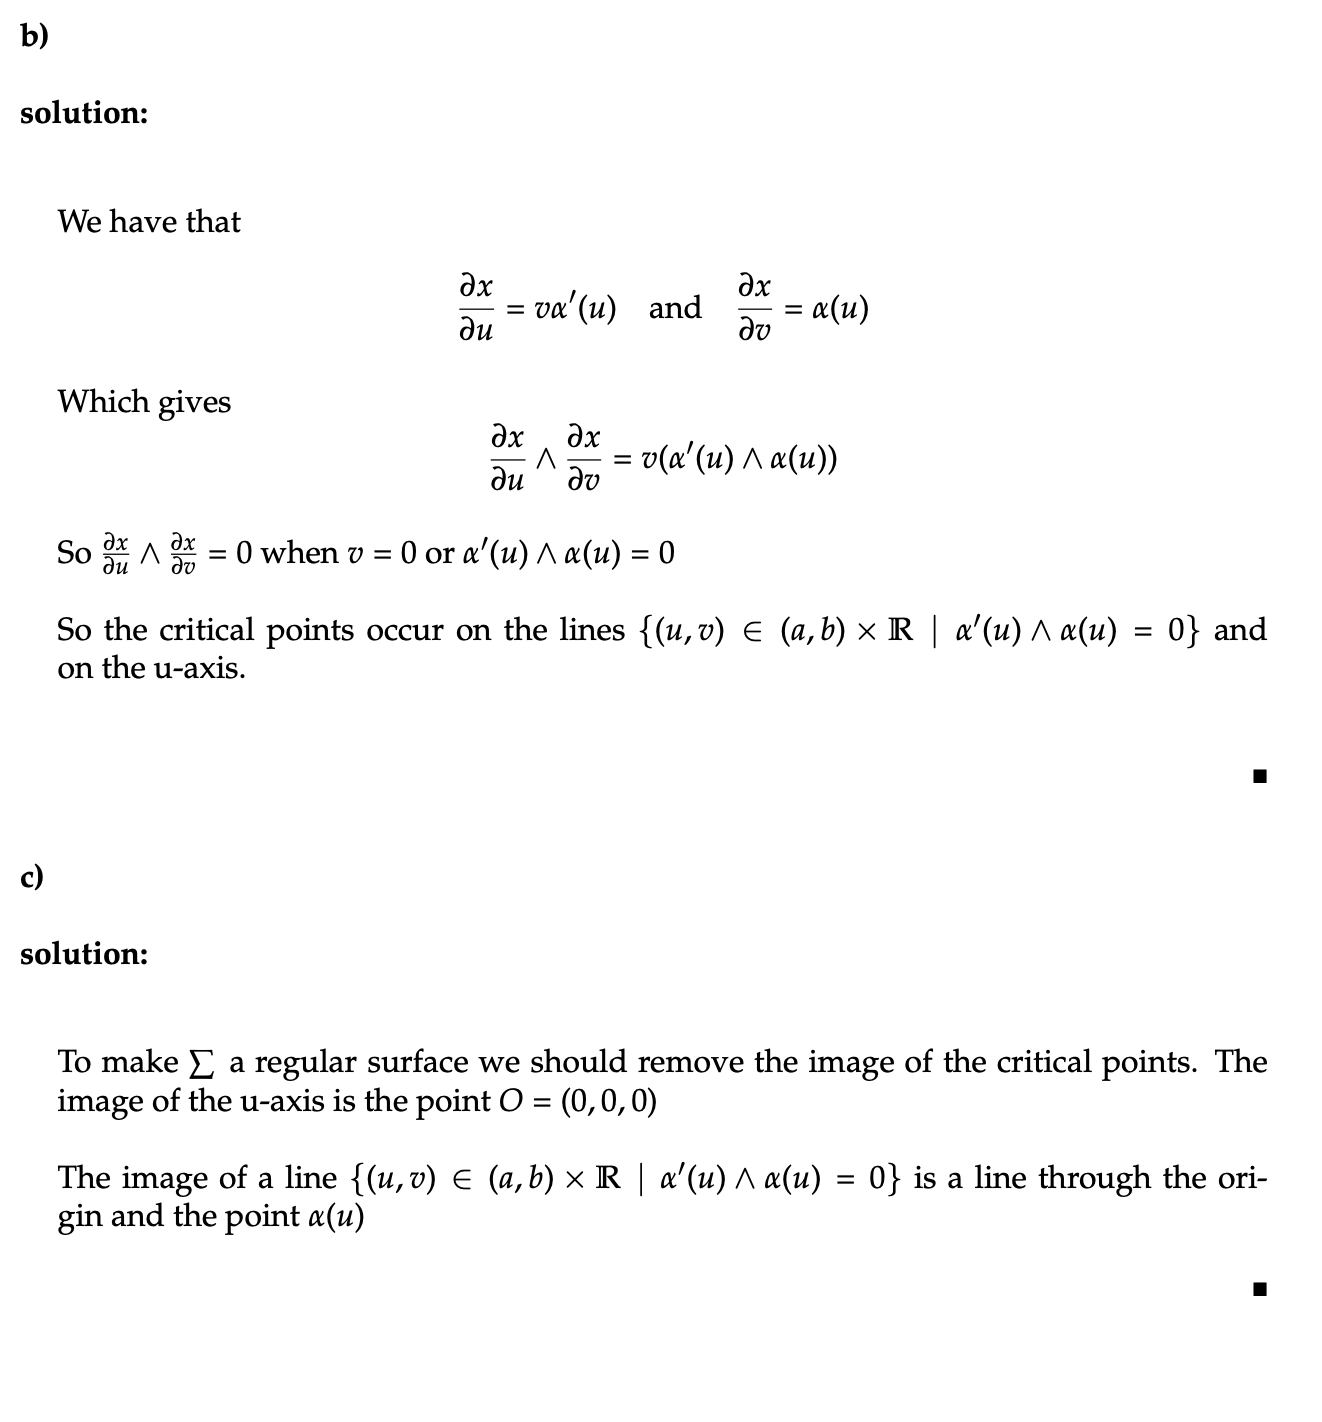
\includegraphics[scale=.8]{C_f2_solution.png}
\end{solution}


\newpage 
%\textbf{D: Extra Credit Problems}\\
%\begin{problem}
%Problem 13 on page 82, Section 2-3, Baby Do Carmo.
%
%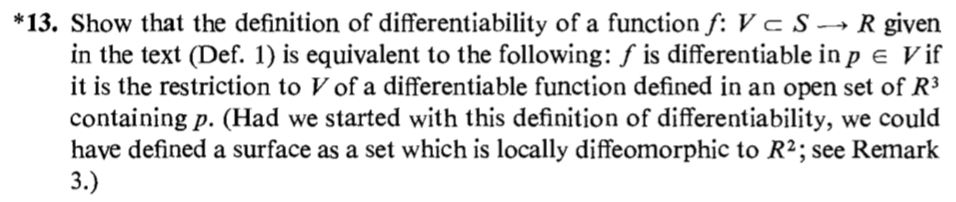
\includegraphics[scale=0.7]{D.png}
%\end{problem}
%\begin{solution}
%\end{solution}

\begin{problem}
  g) Problem 15 on page 82, Section 2-3, Baby Do Carmo. \\

  
\end{problem}
\begin{solution}
  a) It was shown in the book that all parameterizations of a surface are
diffeomorphic to one another and for any parameterizations $\alpha, \beta$, $\alpha^{-1} \circ
\beta$ is diffeomorphic. \\
b) \\
\begin{align*}
  |\int_{\tau_0}^{\tau} |\beta'(\tau)| d\tau| &= |\int_{\tau_0}^{\tau} |(\alpha \circ h)'(\tau)| d\tau| \\
  &= |\int_{t_0}^t |(\alpha)'(t)| dt|
\end{align*}

\end{solution}
\end{document}

